% Slug: four-of-diamonds
% Description: ?
% Author: Cisco
% Story: Cisco
% Test Data: Cisco
% Testers: ?
% Editorial: ?
% TempSlug: four-of-diamonds

% Please don't modify or delete TempSlug

\problem{Tetris Fanfiction}
A \textit{tetromino} is a shape formed by connecting four unit squares together edge-to-edge.  If we count rotations as fundamentally the same shape (but reflections are distinct!), then there are \textit{seven} different tetrominos, illustrated below.  Each is commonly associated with an uppercase English letter whose shape it resembles.
\begin{center}
    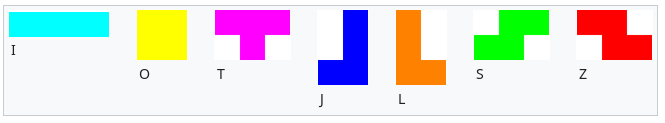
\includegraphics[width=0.75\linewidth]{img/tetris.png}

    \textit{Image taken from Wikipedia}
\end{center}

Tetris is a game in which you are randomly given tetrominos one at a time, and must place them onto to the gameboard in the order you receive them.

Did you know that each next tetris piece is not generated independently from the others?  The sequence of tetris pieces is generated according to the ``7-bag'' algorithm described as follows.  Begin with an empty sequence, then repeat this infinitely many times:
\begin{itemize}
    \item Among all possible permutations of the seven tetrominos, select one of them uniformly at random (this is a ``7-bag'').
    \item Then, append these seven tetrominos \textit{in that random order} as the next seven terms of the sequence.
\end{itemize}
This ensures that there will never be ``droughts'' or ``floods'' of a particular piece, along with many other desirable mathematical properties.

For example, the first sixteen tetrominos in a Tetris game might look like this.  For illustration, tetrominos belonging to the same 7-bag are shown grouped together.
\begin{center}
    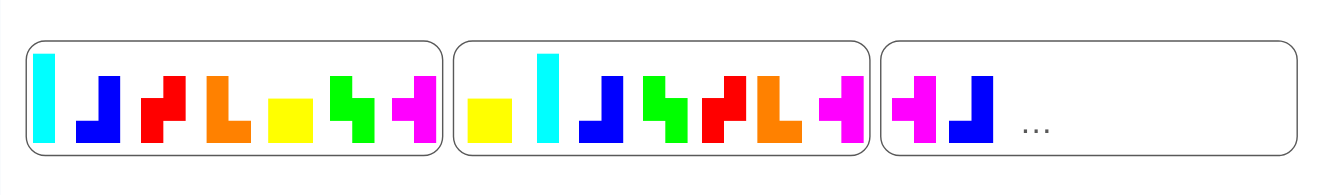
\includegraphics[width=0.95\linewidth]{img/tetris-bag.png}
\end{center}

Bob is writing some Tetris fanfiction, and wants to include the following scene:
\begin{itemize}
    \item \textit{Tetra started a game of Tetris and played for some unknown amount of time.  She paused the game.  Then, when she resumed, we observed that the pieces she got were $t_1$, then $t_2$, then $t_3$, and so on, until $t_n$.}
\end{itemize}
Bob cares about his story being accurate to the game mechanics of real life Tetris.  Is it possible for the sequence $t_1, t_2, t_3, \dots, t_n$ to appear consecutively somewhere in some sequence generated by the 7-bag algorithm?  And if not, what is the fewest number of terms that need to be changed in order to make it so?

\newpage

\subsection*{Input Format}

Input consists of a single line containing a string of $n$ uppercase English letters, each one of \texttt{IJLOSTZ}, where the $i$th letter in the string identifies the tetromino $t_i$.

\subsection*{Output Format}

Output a single integer, the fewest number of terms that need to be changed in order for Bob's sequence to have the desired property.  Note that if it already does have the desired property, you should output $0$.

\subsection*{Constraints}

\textit{Your program will only be tested on data that satisfies the following constraints.}

% Set to 10^5 in true bounds
\constraints{
    $1 \leq n \leq 100$ \\
    Each letter is one of \texttt{IJLOSTZ} \\
}

\textit{There is no need to validate in your program that these constraints hold.}

\subsection*{Sample I/O}

\begin{sampleIO}
\begin{verbatim}
TOIJSZLTT
\end{verbatim}
&
\begin{verbatim}
0
\end{verbatim}
\end{sampleIO}

\begin{sampleIO}
\begin{verbatim}
ZZZZ
\end{verbatim}
&
\begin{verbatim}
2
\end{verbatim}
\end{sampleIO}

\begin{sampleIO}
\begin{verbatim}
TILLJOLTLILTLOSTZITI
\end{verbatim}
&
\begin{verbatim}
4
\end{verbatim}
\end{sampleIO}



\subsection*{Explanation}
In the first sample input, the sequence already has the desired property.  The first \texttt{T} was the last tetromino of the previous bag.  Then, the next bag had the tetrominos in the order \texttt{OIJSZLT}.  Finally, the last \texttt{T} was the first tetromino of the next bag.

In the second sample input, we can make the sequence have the desired property by, for example, changing the last two letters to \texttt{I} and \texttt{O}.